\chapter{Introduction}
\label{sec.introduction}
As home broadband Internet access is rapidly evolving, broadband networks 
have attracted interests from researchers, policy makers and Internet 
Service Providers (ISPs). The United States alone has more than 279 million 
broadband users and number of Internet users in other regions are even more 
impressive: China has more than 641 million Internet users and other 
developing countries are seeing increased growth~\cite{asia}. Despite their 
pervasiveness, little is known about most home networks hampers progress in 
a number of important research areas, from ISP performance to large-scale 
topology mapping and wireless network utilization. In addition, smart home is now an exciting reality. In 2016, 4 billion new ``things" will become available to consumers~\cite{gartner}. For these devices to work, they usually need connect to home wireless router. It is possible that hackers are able to open your front door via a buggy software in home wireless router. Therefore, understanding what the vulnerabilities are and preventing these attacks must be considered.

Currently it has been difficult to study home networks on a large scale because network technologies like network address translators (NATs) present only an opaque view of the home network to the global Internet. To better understand home networks, an experimental platform should be hosted in home networks, to provide visibility into the missing part of Internet. Such a platform also should provide a set of programming interfaces that support the implementation of as wide an array of measurement as possible without compromising the privacy of the user and abuse of host or network resources. 

Today's measurement and experimentation platform for home networks such as 
BISmark~\cite{183951}, Samknows~\cite{samknows} and Dasu~\cite{
sanchez2014measurement} all support controlled network experimentation 
and broadband characterization. However, the process of vetting BISmark 
experiments is manual, which will be a limiting factor as the deployment 
grows. SamKnows has deployed thousands of home routers in the US and the UK, 
but only supports limited performance measurements. Dasu is a host-based 
software client, thus it is not able to run certain measurements due to 
application restriction and cannot run continuous measurements (i.e., since 
hosts can be turned off, moved, etc.)
 
To address these issues, we developed \sysname, an open research testbed that implements a number of measurements primitives that enable researchers, policy makers and Internet Service Providers (ISPs) to program network measurements. \sysname is able to deploy on home wireless router so that it is capable of running both active and passive experiments from a vantage point between the access ISP and the home network, as shown in Figure~\ref{figure:design}. To ensure safety, \sysname supports a very flexible language for experiment specification based on Repy which is lightweight, python based, performance isolation and extensible programming language~\cite{cappos2010retaining}. It provides researchers with the ability to install sandboxed measurement applications on the home wireless router. 

\begin{figure}%[h]
\centering
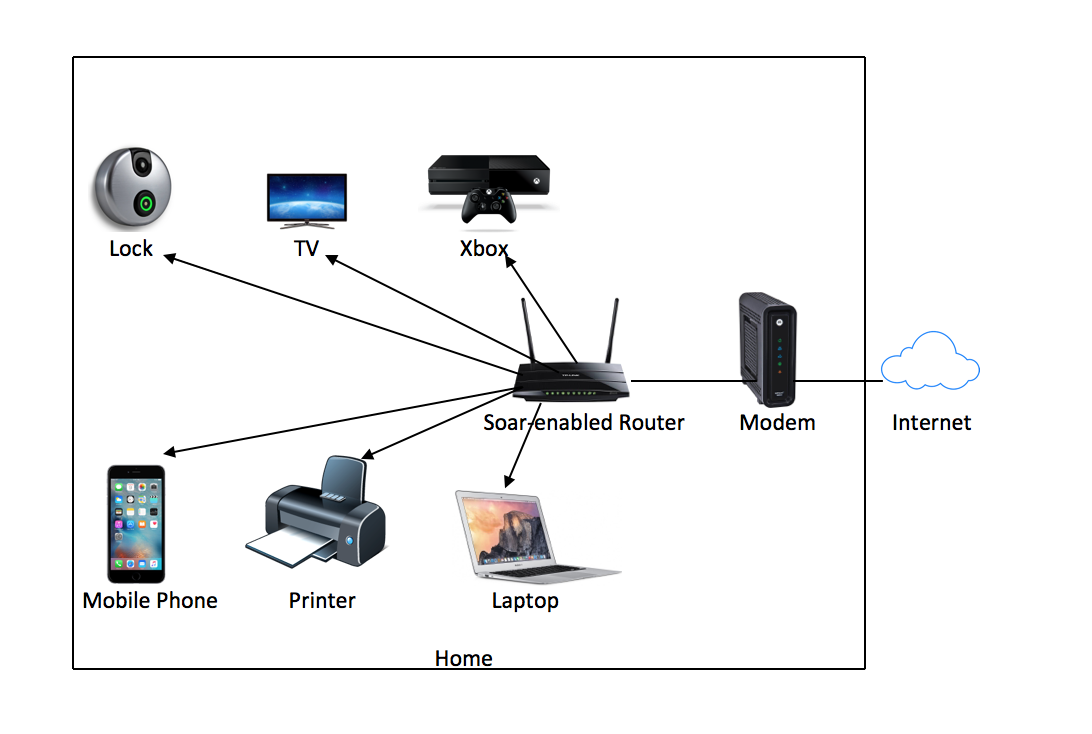
\includegraphics[width=0.8\columnwidth]{figure/home-network.png}
\caption{The Soar-enabled router sits on the direct path of real 
Internet users. It collects both active and passive measurements.}
\label{figure:design}
\end{figure}

Both strengths and challenges of a platform like \sysname stem from 
its inclusion of measurement softwares on the home gateway. First, each softwares must be small and easy-to-deploy because \sysname is deployed on resource-constrained devices. Second, \sysname softwares are on the direct path of real Internet users. Thus it must guarantee the safety of the volunteer nodes. Third, it is important to make system robustness, remote maintenance and update because of the unmanaged complexity of its home network environments. Finally, \sysname must provide a rich set of APIs for a variety of network measurements.

In this paper, we introduce \sysname, a distributed cloud platform that allows researchers to run their project on system worldwide. This testbed provides secure data access while preserving user's privacy. Through a programmable interface on device, the testbed enables researchers to deploy a wide range of network measurements including active and passive measurements. We also discuss the constraints we faced in the design, implementation and deployment of \sysname. 

We make the following contributions in this work:
{\raggedright
\begin{itemize}
\item\textbf{1) Home routers platform deployment:} This platform is based on Seattle testbed~\cite{zhuang2013experience}~\cite{cappos2009seattle}, a community-driven, open-source cloud computing system. Compared to computer and mobile device environments, deployment on home wireless router has more resource limitation such as restricted computational resources. However, recently we are able to port Seattle Testbed to OpenWrt, a popular Linux platform for home routers\cite{openwrt}. Users can build their own \sysname installer (IPK) via config file we provide using OpenWrt SDK and install it on the device directly. 
\item\textbf{2) Extensions to Seattle Testbed:}  Our testbed implements new research capabilities for home wireless router by improving on the Seattle sandbox. To handle home wireless routers, our testbed uses low-level system calls in the OpenWrt platform with the Restriction Python (Repy)\cite{cappos2010retaining}, the core sandbox of Seattle. In order to securely interact with home routers on remote user devices, we use Fence~\cite{li2015fence} to allocate a fixed percentage of the device's CPU, memory disk, and other resources to one or more VMs. For example, we set the legal times of accessing \texttt{/proc} file system to prevent DoS attack using our API calls. Our testbed adds eight functionalities based on Repy, include \texttt{get\_network\_bytes}, \texttt{get\_network\_packets}, \texttt{get\_network\_interface}, \texttt{wifi\_status}, \texttt{scan}, \texttt{get\_station}, \texttt{ping} and \texttt{traceroute}. Through these new functionalities we proposed, researchers are able to implement a wide range of network measurements.
\item\textbf{3) Experimental Characterization of home wireless networks:} By integrating \sysname with the home networks, we get the benefits of a real world deployment while ensuring flexibility to run experiments without compromising home network. We demonstrate \sysname's utility by implementing hybrid measurements that together exercise different new API calls (e.g, \texttt{get\_network\_bytes}, \texttt{get\_network\_interface}, \texttt{wifi\_status}): Characterizing home wireless performance from gateway view. We monitor our lab's network traffic which in an office building from the vantage point of the gateway. We report on additional experiences gained using \sysname in three different use cases. We find that there are many factors affecting throughput on 2.4 GHz and 5 GHz band. We also find that most of access points use non-overlapping channels (e.g., channel 1, 6, 11). 
\end{itemize}
\par}
The rest of thesis is structured as follows: We provide background and motivation in \S{\ref{sec.background_motivation}}. \S{\ref{sec.design}} and \S{\ref{sec.implementation}} describes the design and implementation of \sysname and characterize our current deployment. We present three study cases to illustrate the benefits of an experimental platform that runs on the home wireless router in \S{\ref{sec.evaluation}}. Finally, we discuss future work and conclusion in \S{\ref{sec.conclusion}}. 